\documentclass[convert={size=320x320}]{standalone}
\usepackage[utf8]{inputenc}
\usepackage{tikz}
\usetikzlibrary{calc, decorations.markings}
\usepackage{siunitx}
\sisetup{locale=FR, per-mode=symbol}

\begin{document}
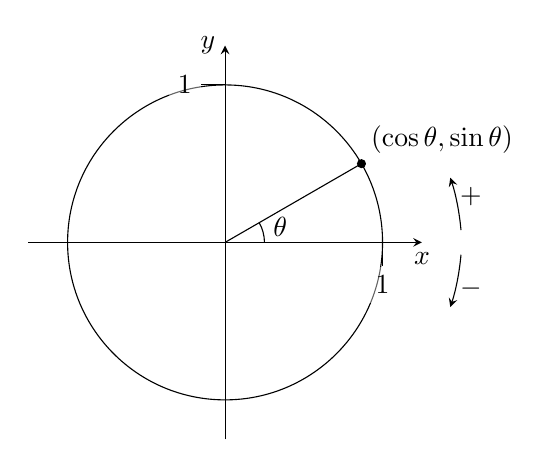
\begin{tikzpicture}[>=stealth]
  \def\radius{2}
  \def\angle{30}
  \coordinate (O) at (0, 0);
  \coordinate (A) at ($(O) + (\angle:\radius)$);
  \draw (O) circle(\radius);
  \draw[->] (-\radius - 0.5, 0) -- (\radius + 0.5, 0) node[below] {$x$};
  \draw[->] (0, -\radius - 0.5) -- (0, \radius + 0.5) node[left] {$y$};
  \draw (O) -- (A);
  \node[anchor=south west] at (A) {$(\cos\theta, \sin\theta)$};
  \draw[fill=black] (A) circle (0.05);
  \draw ($(O) + (0.5, 0)$) arc (0:\angle:0.5);
  \node at (0.7, 0.2) {$\theta$};
  \draw (\radius, 0) -- (\radius, -0.3) node[below, fill=white, fill opacity=0.4, text opacity=1] {$1$};
  \draw (0, \radius) -- (-0.3, \radius) node[left, fill=white, fill opacity=0.4, text opacity=1] {$1$};
  \draw[->] (3:1.5*\radius) arc (5:18:1.5*\radius) node[anchor=north west] {$+$};
  \draw[->] (-3:1.5*\radius) arc (-5:-18:1.5*\radius) node[anchor=south west] {$-$};
\end{tikzpicture}
\end{document}
